%!TEX root = ../main.tex
%%

\chapter{Background}
\section{Datasets}
The data to be learned from is central to any machine learning task. Image datasets can range from hundreds to millions of instances, and can encompass any number of depicted classes from one to tens of thousands. Image data is usually subject to some form of preprocessing due to practical constraints: inputs to any neural network are required to be of fixed dimensionality and these dimensions cannot be excessively large (like high-resolution images). This usually leads to the resizing of images to fit as in \cite{Krizhevsky-2012}, where images were downsampled to 256x256 pixels, and \cite{LeCun-1998}, where the dataset was normalised to contain only 28x28-pixel images. \\

The dataset resulting from \cite{LeCun-1998}, MNIST, is ubiquitous in the field of machine learning. Containing 70,000 images, MNIST is small by comparison to modern datasets such as ImageNet, but its features (handwritten digits) are simple, and a modern network can be trained to near human-level performance on it (\cite{Krizhevsky-2012}). Contemporary datasets are orders of magnitude larger and contain far more complex features than older ones such as MNIST: ImageNet (\cite{imagenet_cvpr09_orig}) is a dataset of over 15 million high-resolution images depicting 22,000 distinct object categories. \\

The dataset used by this project (henceforth 'Micropics') is that used in the Micropics project\footnote{GitHub - pamelaajohnston/micropics. (no date). Available at: https://github.com/pamelaajohnston/micropics (Accessed: 19/11/2021)}. It comprises 311 microscope images of the cyanobacteria \textit{Aphanizomenon flos-aquae}. Each of the dataset's images has both an original and annotated version (where the ground truth of each cell's location in the image is annotated by a red dot). Compared to ImageNet, which contains a huge variety of raw and processed images taken by different cameras and with different styles, Micropics' images are taken under controlled conditions and are all highly similar. They also depict a single object class, the cells themselves. In the respect of being a relatively small and feature-limited dataset, Micropics is similar to the dataset used in \cite{xie2018microscopy}, which is a synthetic dataset created by \cite{Zisserman} (using the method described by \cite{Computational-framework}). This dataset comprises 200 images, and of these, random subsets of only 8 and 64 were used for training, with a further 100 for testing. The results of \cite{xie2018microscopy} from such a small dataset are promising for the few-shot learning that will be inevitable in this project due to the diminutive size of Micropics. The Micropics dataset is likely to be subject to a standard 70/30 or 80/20 split, but the effects of other splits could be explored.\\

\begin{figure}[h!]
	\centering
	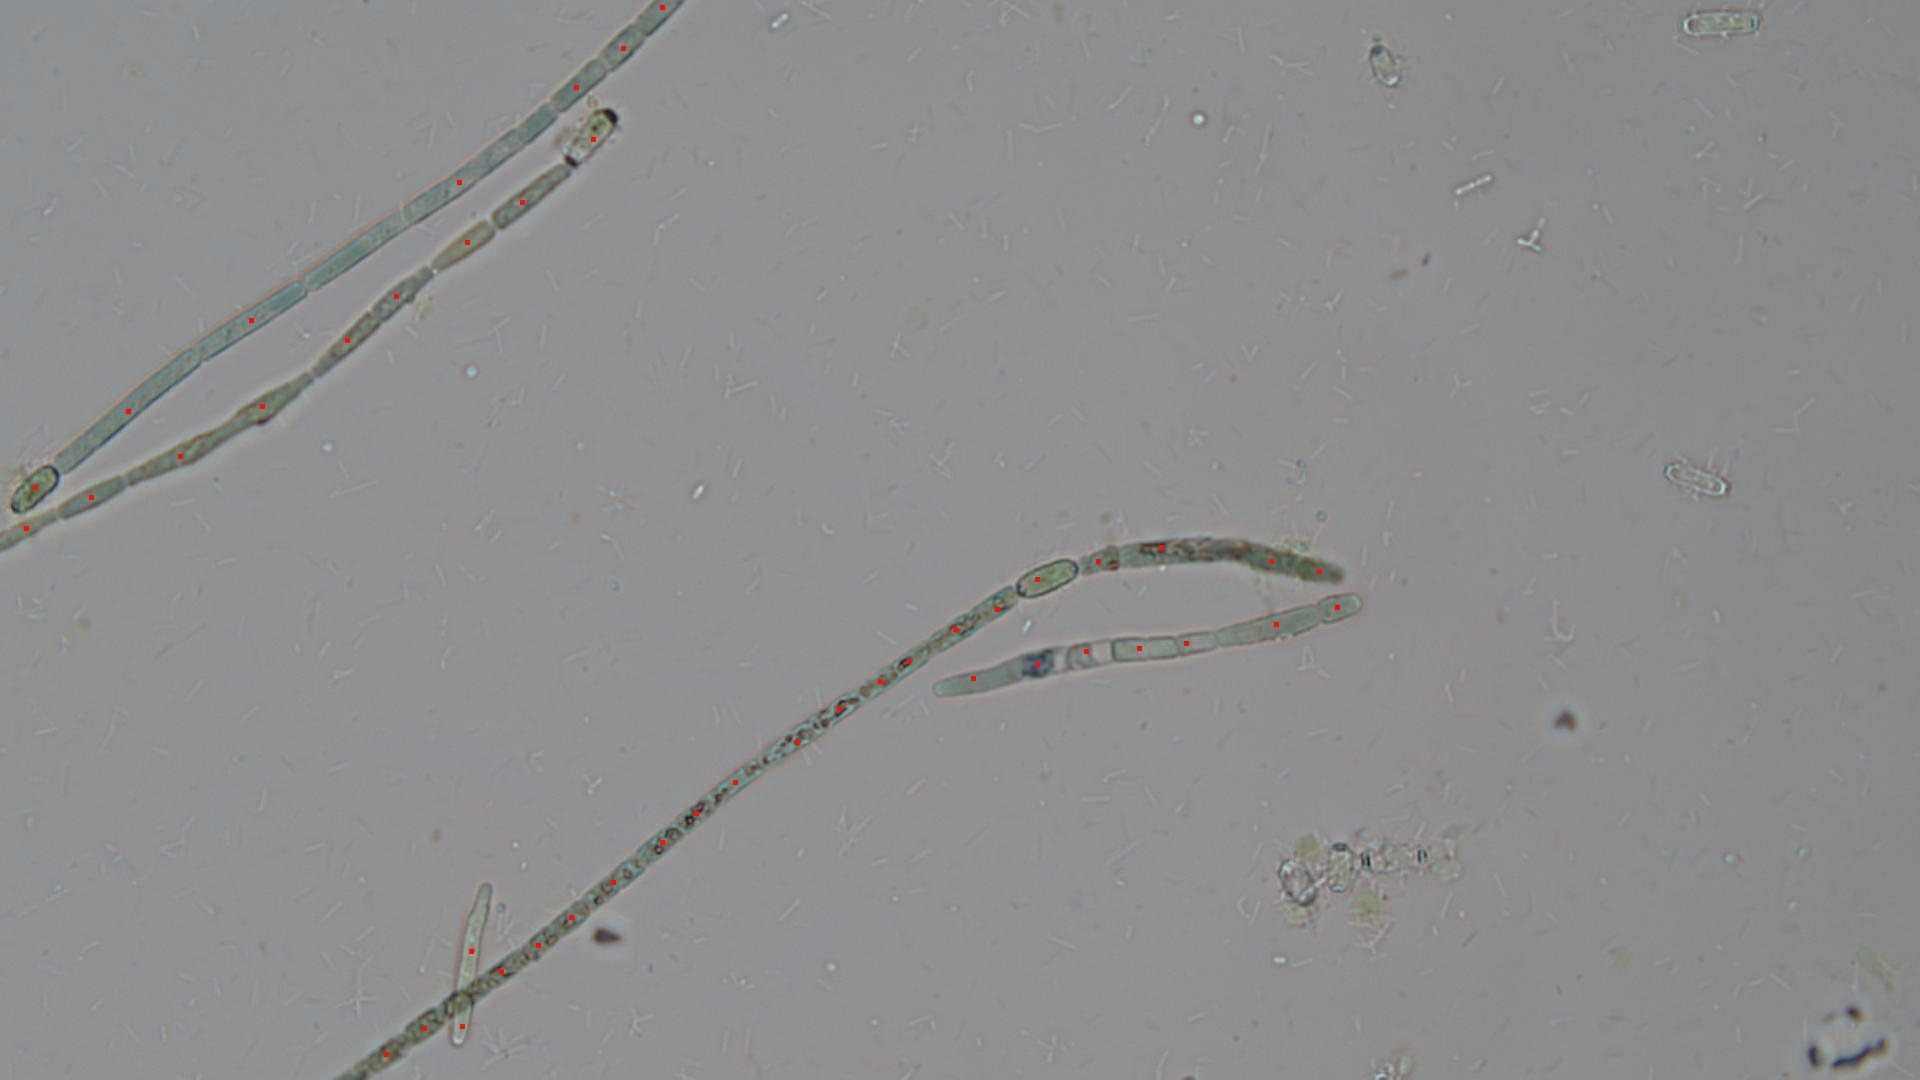
\includegraphics[width=0.5\textwidth]{images/02Background/micropics.jpg}
	\caption{An example of an annotated image from the Micropics dataset (red dots for ground truth)}
\end{figure}

In their unprocessed form, the images are unsuitable for learning due to their high resolution (1920x1080), so they must be either downsampled or converted to cropped patches. Downsampling an image necessarily causes information to be lost, and in the case of the images in Micropics, the objects to be counted are particularly small within the image, which is known to cause detection networks to fail (\cite{redmon2016look}); this problem would be exacerbated by downsampling. The ground-truth annotation dots (which are themselves part of the images) might also be blurred or made inconsistent by downsampling and antialiasing (which is a by-product of, for example, the downsampling method used in \cite{LeCun-1998}). Some networks such as YOLO (\cite{redmon2016look}) predict a limited number of objects per region of an image, and the images in Micropics depict close clusters of small objects, which YOLO is known to struggle with. Hence the decision to segment the images into size-normalised patches appears to be the best choice for the use case, an approach also taken by \cite{xie2018microscopy}.

\section{Convolutional Neural Networks}
The roots of the neural cell counting project are inseparable from those of neural networks themselves. These can be traced as far back as the first convolutional neural networks, which enabled the development of generalisable neural models for image recognition, localisation, and counting (\cite{LeCun-et-al-2015}).\\

The fully-connected neural network (NN) architecture is of limited use for processing images. These networks simply take an input image as a 1-dimensional vector of pixels, and propagate this through each fully-connected layer. This ignores the strong 2-dimensional structure of images, where pixels that are close together are strongly correlated, and local groups of pixel values can yield important patterns and features that are useful for identification. NNs also have no in-built tolerance for variations in position and size or distortions of features in images (\cite{LeCun-et-al-2015, LeCun-1998}). The development of Convolutional Neural Networks (CNNs) was motivated by the search for this region-invariant, feature-based detection, and inspired in part by the findings of \cite{hubel1962receptive}, who found that the visual cortex of cats was composed of ‘simple’ and ‘complex’ cells. Both types of cells detect edges and bar patterns with specific orientations, but while 'simple' cells detect these patterns only at specific locations, 'complex' cells are indifferent to the whereabouts of the pattern in the visual field. \cite{hubel1962receptive} proposed that 'complex' cells simply combined inputs from a number of 'simple' cells that detected the same pattern, but at different regions in the visual field, to produce their region-invariant properties. This concept that several 'simple' feature detectors can be summed to detect more 'complex' features is the underlying assumption of CNNs.\\

CNNs subject the input image to a process of ‘convolution’ which can extract the features of an image. A convolutional layer is a grid of neurons, the inputs to each of which are the units from a small neighborhood ('receptive field') in the previous layer (or the input image). Taking contextual inputs in this form allows the neuron to learn local features in an image. At the first convolution layers these features are simple edges and corners. Subsequent layers combine these simple features to learn higher-level ones. Since the neurons in a convolutional layer all share the same set of weights, they can detect features regardless of whether its location, size etc. in the input image changes (\cite{LeCun-1989}).\\

\begin{figure}[h!]
	\centering
	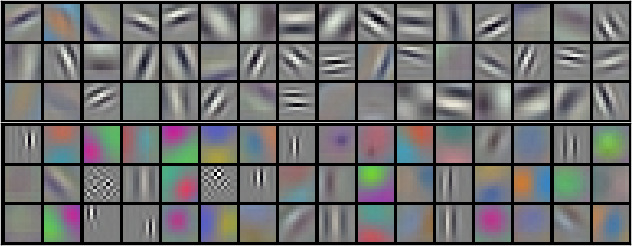
\includegraphics[width=0.5\textwidth]{images/02Background/filters.jpg}
	\caption{Features learned by the first convolutional layers of AlexNet (\cite{Krizhevsky-2012})}
\end{figure}

\cite{FUKUSHIMA1982455}'s Neocognitron was an early ancestor of the modern CNN which took direct inspiration from \cite{hubel1962receptive}. The Neocognitron was comprised of several modules, each containing a first layer of 'S-cells' connected to a second of 'C-cells'. These 'C-cells' achieved some success in digit recognition, but the Neocognitron relied upon an inferior, unsupervised reinforcement algorithm for training, since it was conceived before the development of the fully supervised backpropagation learning that would later enable remarkable achievements by CNNs.\\

Due to their proven track record (\cite{Krizhevsky-2012,girshick2014rich,redmon2016look}), CNNs are the network architecture of choice for reliable object detection in images (\cite{LeCun-et-al-2015}). CNNs are also broadly applied to automated counting applications, including the counting of cells; \cite{xie2018microscopy} and \cite{Identification-and-enumeration-of-cyanobacteria} both use CNN-based approaches to counting cells, even where cells are not individually detected, as in the case of \cite{xie2018microscopy}. Being the predominant method for object recognition and counting, there is a wealth of CNN-based image recognition and counting literature and software to learn from and build upon in the development of a new cell counter, making it the natural choice for further investigation.

\section{Detection}
Before cells can be counted, they must be detected. CNNs have been applied with great success to generalised object detection, and their feature-based learning holds promise for the task of detecting and counting cells.\\

\subsection{LeNet}
What became LeNet-5 was in development for nearly 10 years from 1989 to 1998. \cite{LeCun-1989} pioneered the first multi-layered CNNs and applied them to the task of image recognition, in LeNet’s case handwritten character recognition. By 1999 LeNet-5 was reading 10\% of all cheques in the U.S. (\cite{LeCun-et-al-2015}). \cite{LeCun-1989} makes reference to Fukushima’s Neocognitron, from which it takes inspiration for the network's convolutional architecture, but emphasises LeNet’s fully supervised learning using backpropagation and stochastic gradient descent, which freed LeNet from the highly problematic and difficult manual preprocessing that characterised previous attempts at feature extraction (\cite{LeCun-1989,8016501}). Using backpropagation, LeNet could learn the required features automatically.

\subsection{AlexNet}
After the early successes of LeNet, the use of CNNs stagnated through the 2000s, but the ImageNet 2012 competition could be credited with kick-starting the contemporary renaissance of interest in image recognition using CNNs (\cite{LeCun-et-al-2015}). On the ImageNet LSVRC-2010 dataset—a set of 1.2 million images together depicting 1000 distinct object classes—AlexNet, the model described in \cite{Krizhevsky-2012}, achieved a ‘top-1 error rate’ of 37.5\% (where the most confident class predicted by the model is incorrect), and a ‘top-5 error rate’ (where the correct class is not present in the model’s top 5 predictions) of 17.0\%. These scores defined the state of the art at the time, and AlexNet went on to win the LSVRC-2012 competition with a top-5 error rate of 15.3\%, more than 10\% less than the second-place model.\\

This unprecedented performance can be attributed to several innovations in AlexNet. At the time of this achievement the \textit{de rigeur} neural activation functions for hidden units in a network were the hyperbolic tangent \(f(x) = tanh(x)\) and logistic sigmoid \(f(x)=\sigma(x)\) \cite[p. 191]{Goodfellow-et-al-2016}). LeNet as an example used \(tanh\) as its activation or ‘squashing’ function. AlexNet conceived of applying the Rectified Linear function \(f(x)=max(0,x)\) to this purpose, creating a network of Rectified Linear Units (ReLUs). This circumvents two key weaknesses suffered by \(tanh\) and sigmoid. The first is that the \(tanh\) and sigmoid functions are relatively computationally intensive compared to the exceedingly simple ReLU. With a dataset as large as ImageNet this results in a severe upper limit on the size of a network that could be trained on the data, due to excessively high training times. ReLU also allowed the network to avoid the second weakness suffered by \(tanh\) and sigmoid, the well-documented ‘Vanishing Gradient’ problem (\cite{Dying-ReLU}), where at high or low input values, the gradient of tanh and sigmoid is close to zero and provides little to no useful information to influence the model during backpropagation. This innovation allowed AlexNet to train on ImageNet 6 times faster than an equivalent network using \(tanh\) units, enabling it to train to an exceptionally high accuracy. It also made use of a regularisation technique known as 'Dropout', new at the time, which randomly and temporarily deactivates a proportion of the units in the network when training on a new image. This ensures that units do not become reliant on the presence of other units, and a unit must therefore learn features that are useful with \textit{any} configuration of the other neurons in the network. This method makes AlexNet resilient against overfitting.\\

The legacy of AlexNet is broad and deep. The use of the once-ubiquitous \(tanh\) and sigmoid activation functions is now discouraged \cite[p. 191]{Goodfellow-et-al-2016}, and ReLU (and its derivatives such as LeakyReLU) has become a default choice for modern neural networks. While AlexNet is now an antiquated network, it laid the groundwork for many successors (\cite{redmon2016look}'s YOLO uses both a ReLU-derived activation function and Dropout) which have been applied to all manner of tasks, not only object detection but also object localisation and counting.

% At high or low input values, the gradient of both functions is close to zero and provides little to no useful information to influence the model during backpropagation when the function is derived. ReLU’s linearity above 0 means it never ‘saturates’ at higher values, i.e., its gradient does not level off. The ‘non-saturating’ property attributed to the neurons in AlexNet is in reference to this, and it means the units do not suffer from vanishing gradients at higher values during learning.

% \cite{Krizhevsky-2012} omits to mention that ReLU \textit{does} inherently suffer from the vanishing gradient problem at values below zero: since the gradient below zero is zero, if ReLUs are subjected to negative inputs they may fall into a state where they only output zero for any input and cannot be recovered, becoming ‘dead’ and of no use to the network. This is a well-understood issue known as the ‘Dying ReLU’ problem (\cite{Dying-ReLU}). The dying ReLU problem has since been addressed in various ways, including various hand-designed and generated functions intended to supersede it, but as noted by \cite{Searching-for-Activation-Functions}, the plethora of functions proposed to supersede ReLU show inconsistent performance across different tasks and datasets. Many also introduce further complexity to the process of training the network in the form of an extra parameter to be tuned. Nonetheless, the use of the once-ubiquitous tanh and sigmoid activation functions is now discouraged \cite[p. 191]{Goodfellow-et-al-2016} and while ReLU has become a 'default' choice for modern neural networks (\cite{Goodfellow-et-al-2016,Searching-for-Activation-Functions}), optimising activation functions remains an open question.

\section{Localisation}
Detecting cells is a prerequisite to \textit{localising} each cell in an image. The images in Micropics are annotated with this in mind: the location of each is denoted by a dot annotation. Once the location of all cells is known, counting is trivial. Several techniques exist for object localisation in images.

\subsection{R-CNN \& Derivatives}
R-CNN (\cite{girshick2014rich}) was introduced as an adaptation of the CNN for object localisation rather than classification. Given an input image, R-CNN generates around 2000 'region proposals' or 'regions' from the image (each itself an image), based on which areas are deemed likeliest to contain an object. In \cite{girshick2014rich} this is determined by the selective search algorithm, although there are many other algorithms for region proposal and the network is agnostic to the algorithm used. Each region proposal is category-independent, not referring to any particular object class. Subsequently, each region is resized and forward-propagated through a deep CNN (an implementation of AlexNet with no classification layer). This results in a 'feature vector' for each region proposal. Finally, each feature vector is classified using a Support Vector Machine and each region proposal assigned a confidence score, and the scored regions are distilled by discarding the lower scoring region where any two regions containing the same class are overlapping.\\

\begin{figure}[h!]
	\centering
	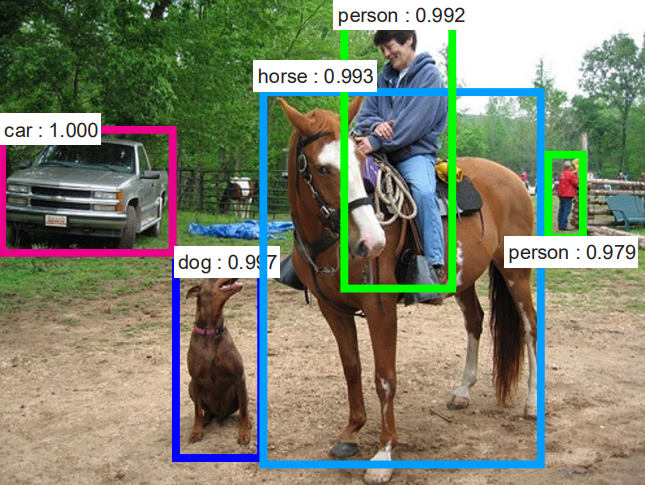
\includegraphics[width=0.5\textwidth]{images/02Background/rcnn.png}
	\caption{An image processed by Faster R-CNN (\cite{ren2016faster})}
\end{figure}

One disadvantage of the R-CNN system is that it is relatively slow. In \cite{girshick2015fast}, an R-CNN network was found to take 47 seconds to process a single image at test time. This led to the development of Fast R-CNN (\cite{girshick2015fast}), and Faster R-CNN (\cite{ren2016faster}). The former of these achieved 213 times faster test-time processing than R-CNN and higher detection quality. The latter achieved a processing speed of 6 images per second, approaching real-time performance. R-CNN and its derivatives have seen successful applications to the detection of pedestrians (\cite{Fast-CNN-Pedestrians}), faces (\cite{Fast-R-CNN-Faces}), and the counting of cells (\cite{Identification-and-enumeration-of-cyanobacteria}), and a PyTorch-based implementation of Faster R-CNN is available as part of Detectron 2, Facebook AI's object-detection library\footnote{GitHub - facebookresearch/detectron2. (no date). Available at: https://github.com/facebookresearch/detectron2 (Accessed: 19/11/2021).}. Detectron is open-source and development is highly active, making Faster R-CNN a reliable option for a counting project.

\subsection{YOLO}
Following Faster R-CNN, another object-localisation network was developed, realising Faster R-CNN's aspirations for real-time performance: \cite{redmon2016look}'s YOLO. YOLO has the advantage over Faster R-CNN of consisting of only a single component for both detection and localisation, compared with Faster R-CNN's relatively complex pipeline. Compared to the state of the art at the time (R-CNN and derivatives), YOLOv1 made more errors in localising objects, but predicted fewer false positives and maintained a competitive mAP (mean average precision). It also showed a greater ability to generalise than Faster R-CNN. Most crucially, it was capable of processing images at 45 frames per second. YOLO has since been updated several times, and in the task described by \cite{benjdira2018car}, it was shown that YOLOv3 exhibited not only dramatically faster, but also better performance than Faster-CNN.\\

YOLO's remarkable speed makes it more suitable than other networks for experimentation using commercial hardware. The original author (\cite{redmon2016look}) developed YOLO to version 3, but an open-source PyTorch version known as YOLOv5 is currently maintained by Ultralytics\footnote{GitHub - ultralytics/yolov5. (no date). Available at: https://github.com/ultralytics/yolov5 (Accessed: 19/11/2021).}. This is a highly active project, and would serve as a reliable basis for experimentation in applying the YOLO network to the domain of cell counting. Alternatively, an implementation of YOLOv3 is available for Keras \footnote{GitHub - qqwweee/keras-yolo3. (no date). Available at: https://github.com/qqwweee/keras-yolo3 (Accessed: 19/11/2021).}.

% AlexNet popularised the use of ReLUs, but YOLO takes this a step further by using a network of LeakyReLUs. LeakyReLU is linear for inputs above zero, but for inputs below zero returns the input multiplied by a (small) value \(\alpha\), creating a small gradient. LeakyReLUs always return some gradient, which mitigates the ‘Dying ReLU’ problem caused by ReLU’s vanishing gradient below zero. However as previously noted in \cite{Searching-for-Activation-Functions}, ReLU-derived functions such as LeakyReLU do not reliably generalise to all tasks and there is scope to explore the effects of the activation function as an additional network parameter.

\section{Counting} \label{density-estimation}
If a network can detect and localise cells in an image, counting the cells becomes trivial (\cite{Zisserman}). However, direct detection of individual objects is not the only method available for counting, and another method known as 'density estimation' has also been applied to the domain of cell counting.

\subsection{Detection vs. Density Estimation}
R-CNN and other detection-based methods have been shown to produce reliable counts from images; \cite{Identification-and-enumeration-of-cyanobacteria} uses it to localise and count cyanobacteria cells. While detection-based counting can be highly effective, the efficacy of object detection tends to degrade when objects are occluded or overlapping (\cite{Zisserman}). An alternative method of obtaining a count of objects is to estimate their density in an image. This is done by learning a \textit{mapping} between the global features of an image and a count of the objects depicted by it. This is the approach taken by \cite{xie2018microscopy}. Both \cite{Zisserman}  and \cite{xie2018microscopy} use images whose ground truth is provided by by dot annotations at the locations of objects (as in the Micropics dataset). The system then learns a density map from the features of the image that is trained to match the ground truth as closely as possible.\\

\begin{figure}[h!]
	\centering
	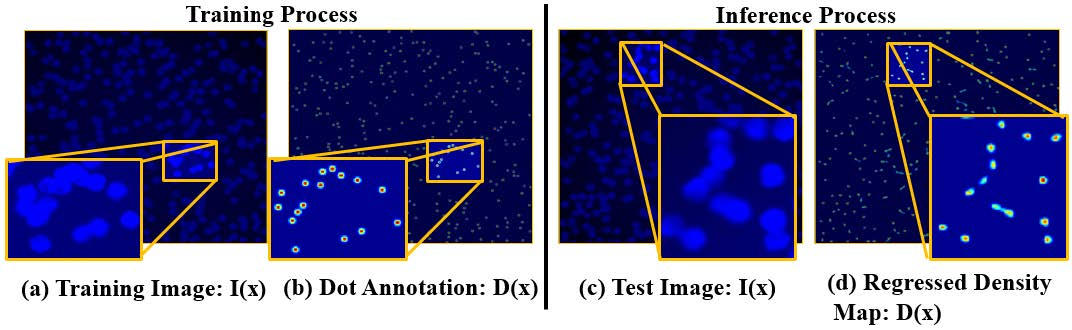
\includegraphics[width=0.5\textwidth]{images/02Background/density.jpg}
	\caption{An example of a learned density map (\cite{xie2018microscopy})}
\end{figure}

Existing density estimation-based counting methods, while achieving success in cell counting, have so far been tested on images (synthetic or otherwise) of cells which are non-filamentous; the structure of filamentous bacteria such as \textit{A. flos-aquae} is quite different, and it is unclear how a density estimation-based approach would transfer to the task of counting filamentous cyanobacteria. \cite{Liu_2018_CVPR} points out that while the density-estimation method is effective for densely crowded images where detection-based methods struggle, density-estimation approaches equally tend to \textit{over}estimate where the density of objects in an image is sparser. This is certainly the case in Micropics, where the filamentous cells are arranged in long lines, rather than clusters, against an empty background. The viability of density estimation-based counting for filamentous cells remains an open question, and a possible alternative to a detection-based method using YOLO.

\section{Conclusion}
As specified at the outset, the objective of this project is to develop an automatic cell counter for filamentous cyanobacteria. There is sufficient scope to find improvements upon current methodology, since the investigation of current literature revealed questions and avenues for further development. The best model to implement for the purpose of the project appears to be YOLO, which has been demonstrated to be a state-of-the-art CNN for image recognition that is also extremely fast compared to other networks. Being so lightweight, it is feasible that YOLO could run at test time on commercial hardware, but given the potential for repeated training it may be necessary to make use of a GPU provided by the University to train the network. Both PyTorch and Keras options are available, but the PyTorch implementation, being more up-to-date, is the more likely candidate. In the event that a detection-based approach with YOLO similar to \cite{Identification-and-enumeration-of-cyanobacteria} is revealed to be unfeasible, the viability of using a density-estimation approach as in \cite{xie2018microscopy} and \cite{Zisserman} on filamentous bacteria could be further investigated.

\subsection{Evaluation}
The cell counter will be a software artefact with a well-defined goal, making it relatively easy to evaluate. The counter should be capable of accepting unannotated images of \textit{A. flos-aquae} from Micropics and returning a number representing a reliable count of cells in the image. The counter's loss can be defined as the absolute distance between this predicted count and the count of ground-truth dot annotations in the annotated image (which can be retrieved by a Python script present in the Micropics repository). This error can be evaluated against that of existing approaches. Another evaluation metric for the model could be to determine the quality of its predicted bounding boxes versus the ground-truth bounding boxes, by their Intersection Over Union (IOU) (defined as the number of pixels that were correctly predicted divided by the number encompassed by both bounding boxes). However, the error in cell count is the only metric strictly needed to evaluate the artefact.\\

The network loss on both training and test sets should be monitored. Since the dataset is small, splitting it into only test and train sets may be desirable rather than also including a validation set. This introduces the problem that while tuning hyperparameters, the network may overfit on both test and train sets while appearing to improve (\cite{zhang2017understanding}). Ideally the network should be tested on an additional validation set to ensure it is not overfitting. An alternative is to use K-fold cross-validation to ensure the network learns from all examples in the dataset. When the model's loss plateaus, it is likely that it is unable to learn any more information with its current hyperparameters, and some tuning will be required. The network hyperparameters are all the more important given the diminutive size of Micropics, since a smaller latent space means there is greater likelihood of falling into a local minimum. Tuning of hyperparameters such as the batch size, number of epochs, and learning rate (or varying the learning rate over training, to prevent the network from oscillating) would be useful for further evaluation of different network configurations, but in a trained network such as YOLO, the selection of hyperparameters available for tuning is likely to be limited.